\documentclass{beamer}

\usetheme{Stockton}
\usepackage{amssymb,graphicx,amsmath,graphicx,epstopdf,url,enumerate,wasysym}
 %\usepackage{beamerthemesplit} %// Activate for custom appearance

\title{Triangulation of the Cube}
\author{Ben Storlie}
\date{\today}

\begin{document}

\frame{\titlepage}

%\section[Outline]{}
%\frame{\tableofcontents}

\section{Introduction}

\frame{
\frametitle{Triangular Numbers}

Triangular numbers are numbers in the form $\sum_{i=1}^n i $.

If $T_2(n)$ is the $n$th triangular number, then 
\begin{quote}
$T_2(1)=1$\\
$T_2(2)=1+2=3$\\
$T_2(3)=1+2+3=6$\\
$T_2(4)=1+2+3+4=10$\\
$T_2(5)=1+2+3+4+5=15$\\
\end{quote}

\begin{center}
$\begin{array}{ccccccccccccc}
&&&&&&&&&&&&\blacksquare \\
&&&&&&&\blacksquare&&&&\blacksquare&\blacksquare \\
&&&\blacksquare&&&\blacksquare&\blacksquare&&&\blacksquare&\blacksquare&\blacksquare \\
\blacksquare&&
\blacksquare&\blacksquare&&
\blacksquare&\blacksquare&\blacksquare&&
\blacksquare&\blacksquare&\blacksquare&\blacksquare \\
\end{array}$
\end{center}
}

\frame{
\frametitle{Triangular Numbers}

Recall that $T_2(n)=\frac{n(n+1)}{2}$.  This gives us a familiar geometric interpretation of a rectangle sliced in half.

\begin{center}
$\begin{array}{ccccc}
\square&\square&\square&\square&\blacksquare \\
\square&\square&\square&\blacksquare&\blacksquare \\
\square&\square&\blacksquare&\blacksquare&\blacksquare \\
\square&\blacksquare&\blacksquare&\blacksquare&\blacksquare \\
\end{array}$
\end{center}

}

\frame{
\frametitle{Tetrahedral Numbers}

Since $\left({n \choose 2}\right)=\frac{n(n+1)}{2}$, $T_2(n)=\left({n \choose 2}\right)$.

Tetrahedral numbers are the sum of consecutive triangular numbers.  $$T_3(n)=\sum_{i=1}^n T_2(i)$$

Since $\sum_{i=1}^n \left({i \choose 2}\right) = \left({n \choose 3}\right)$, we know that $T_3(n)=\left({n \choose 3}\right)$.
}

\frame{\begin{center}
\includegraphics[width=2.5in]{/Users/Ben/Documents/Thesis/Tetrahedra_in_Cubes/tetrahedronpicture.png}\end{center}
}

\frame{
$$\left({n \choose 3}\right)=\frac{n(n+1)(n+2)}{6}$$

This implies that there is an analogous geometric interpretation to triangular numbers.  That is, a $n \times n+1 \times n+2$ box can be divided into $6$ tetrahedra.

\begin{center} \includegraphics[width=2.5in]{/Users/Ben/Documents/Thesis/Tetrahedra_in_Cubes/math097a.jpg} \end{center}

}

\frame{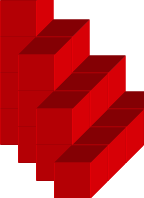
\includegraphics{/Users/Ben/Documents/Thesis/Tetrahedra_in_Cubes/blocks1.png} }
\frame{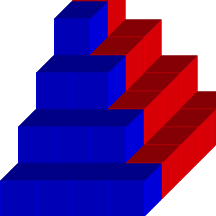
\includegraphics{/Users/Ben/Documents/Thesis/Tetrahedra_in_Cubes/blocks2.png} }
\frame{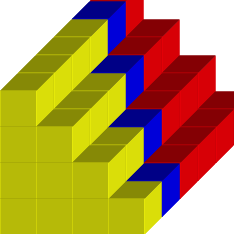
\includegraphics{/Users/Ben/Documents/Thesis/Tetrahedra_in_Cubes/blocks3.png} }
\frame{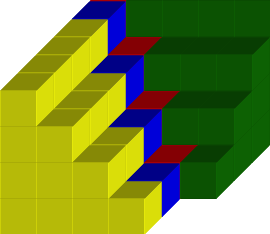
\includegraphics{/Users/Ben/Documents/Thesis/Tetrahedra_in_Cubes/blocks4.png} }
\frame{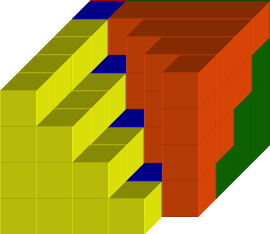
\includegraphics{/Users/Ben/Documents/Thesis/Tetrahedra_in_Cubes/blocks5.png} }
\frame{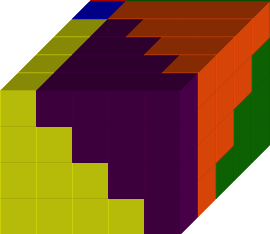
\includegraphics{/Users/Ben/Documents/Thesis/Tetrahedra_in_Cubes/blocks6.png} }


\frame{\frametitle{"Simplexal Numbers"}

We can prove by induction that $$T_k(n)=\left({n \choose k}\right)=\frac{n(n+1)(n+2)\dotsb(n+k-1)}{k!}$$

Which means that geometrically, a $k$-cube can be divided into $k!$ simplices.

How many ways are there to do that?

}







\frame
{
  \frametitle{Parameters}

  \begin{itemize}
  \item <1-> How many ways can an $n$-cube be divided into $n$-simplices?
  	\begin{itemize}
	\item <2-> where each simplex has the same volume,
	\item <3-> and no new vertices are made.\\
		\begin{itemize}
		\item <4-> (i.e. The vertices of each simplex are chosen from the 				vertices of the original cube.)
		\end{itemize}
	\end{itemize}
  \end{itemize}
}
	


\subsection{How Do Simplices Fit into a Cube?}

\frame{\frametitle{How do Simplices Fit into a Cube?}}

\frame{\frametitle{Zero and One Dimensions}
\makebox[2em]{}A point in a point
\centerline{ 
\includegraphics[height=.25 in]{/Users/Ben/Documents/Thesis/Tetrahedra_in_Cubes/simplex1.png}}
\bigskip\bigskip\bigskip
\makebox[2em]{}A line segment in a line segment
\bigskip
\centerline{
\includegraphics[height=.25 in]{/Users/Ben/Documents/Thesis/Tetrahedra_in_Cubes/simplex2.png}}
}

\frame{\frametitle{Two Dimensions}
\centerline{\includegraphics[height=1.9 in]{/Users/Ben/Documents/Thesis/Tetrahedra_in_Cubes/square1.png}}}
\frame{\frametitle{Two Dimensions}
\centerline{\includegraphics[height=2 in]{/Users/Ben/Documents/Thesis/Tetrahedra_in_Cubes/square3.png}}}
\frame{\frametitle{Two Dimensions}
\centerline{\includegraphics[height=2 in]{/Users/Ben/Documents/Thesis/Tetrahedra_in_Cubes/square4.png}}}
\frame{\frametitle{Two Dimensions}
\centerline{\includegraphics[height=2 in]{/Users/Ben/Documents/Thesis/Tetrahedra_in_Cubes/square5.png}}}

\frame{\frametitle{Three Dimensions}
\centerline{\includegraphics[height=2 in]{/Users/Ben/Documents/Thesis/Tetrahedra_in_Cubes/cube1.png}}}
\frame{\frametitle{Three Dimensions}
\centerline{\includegraphics[height=2 in]{/Users/Ben/Documents/Thesis/Tetrahedra_in_Cubes/cube2.png}}}
\frame{\frametitle{Three Dimensions}
\centerline{\includegraphics[height=2 in]{/Users/Ben/Documents/Thesis/Tetrahedra_in_Cubes/cube3.png}}}
\frame{\frametitle{Three Dimensions}
\centerline{\includegraphics[height=2 in]{/Users/Ben/Documents/Thesis/Tetrahedra_in_Cubes/cube4.png}}}
\frame{\frametitle{Three Dimensions}
\centerline{\includegraphics[height=2 in]{/Users/Ben/Documents/Thesis/Tetrahedra_in_Cubes/cube5.png}}}

\frame{\frametitle{Three Dimensions}
\centerline{ A 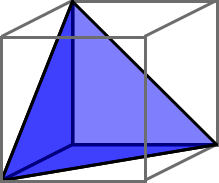
\includegraphics[height=1.2 in]{/Users/Ben/Documents/Thesis/Tetrahedra_in_Cubes/A.png}\quad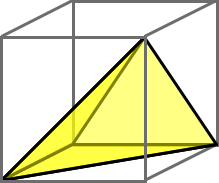
\includegraphics[height=1.2 in]{/Users/Ben/Documents/Thesis/Tetrahedra_in_Cubes/C.png} C}
\bigskip
\centerline{ BL \includegraphics[height=1.2 in]{/Users/Ben/Documents/Thesis/Tetrahedra_in_Cubes/cube3.png} \quad \includegraphics[height=1.2 in]{/Users/Ben/Documents/Thesis/Tetrahedra_in_Cubes/BR.png} BR}
}

\section{How to Fit These Tetrahedra in A Cube}

\frame{\frametitle{Pyramids}
\centerline{  \includegraphics[height=1.5 in]{/Users/Ben/Documents/Thesis/Tetrahedra_in_Cubes/pyramid1.png}\quad\includegraphics[height=1.5 in]{/Users/Ben/Documents/Thesis/Tetrahedra_in_Cubes/pyramid3.png} }

With linear algebra, it can be shown that {\bf A}s and {\bf C}s always come together in pairs like that.  Which means that every tiling with {\bf A} and {\bf C}s in it has a corresponding tiling with only {\bf B}s.
}

\frame{\frametitle{Tilings with only {\bf B} tetrahedra}
Since every {\bf B} tetrahedron has exactly one edge with a $90^\circ$ angle, the problem can be simplified to choosing six edges from the twelve edges of the cube.  Let these chosen edges be called "B edges."

\centerline{
\hfill{}
\includegraphics[width=1.2in]{/Users/Ben/Documents/Thesis/Tetrahedra_in_Cubes/BtetraWithLine1.png}
\hfill
\includegraphics[width=1.2in]{/Users/Ben/Documents/Thesis/Tetrahedra_in_Cubes/BtetraWithLine2.png}
\hfill{}
}

The following rules must be followed when choosing B edges.
\begin{enumerate}
\item Six B edges must be chosen.
	\begin{itemize}
	\item Since $b=6-2a$, and $a=0$, there are exactly six {\bf B} tetrahedra.
	\end{itemize}
\item Each square face must have exactly two B edges.
	\begin{itemize}
	\item Since each square face is made of exactly two triangular faces of {\bf B} tetrahedra.
	\end{itemize}
\item Each vertex can have at most two B edges.
\end{enumerate}
}

\frame{
\includegraphics[width=2.5in]{/Users/Ben/Documents/Thesis/Tetrahedra_in_Cubes/arrangeBs.png}}

\frame{
The above figure shows a two-dimensional projection of the cube.  The edges highlighted blue are where B edges are, and the the edges highlighted green are where B edges \emph{aren't}.

A particular face could have the two B edges being opposite from each other (1) or adjacent (2).  (2) includes an extra green edge because of rule 3.

\begin{itemize}
\item Cube (1) \\
A second face adjacent to the first face can either have the B edges \\adjacent (3) or opposite (4).
\begin{itemize}
\item Cube (3) \\
Rule 2 adds two B edges (6). \\ Rule 2 applied again completes the cube (9).  Cube (9) follows every rule, and so it is valid. $\checkmark$
\item Cube (4) \\
This cube is impossible, by rule 2.
\end{itemize}
\item Cube (4) \\
A green edge is added to make cube (5) distinct from cube (3). \\
A B edge is added by rule 2 (8). \\
A particular face could either have its B edges be adjacent (10) or opposite (11).
\begin{itemize}
\item Cube (10) \\
Rule 2 completes the cube (12).  Cube (12) follows every rule, and so it is valid.  $\checkmark$
\item Cube (11) \\
Rule 2 completes the cube (13).  Cube (13) is equivalent to cube (9), which we know is valid.  $\checkmark$
\end{itemize}
\end{itemize}
}

\end{document}
